\section{GPU Profile}

\begin{frame}{NVIDIA GPU Profiling Tools}
    \begin{itemize}
        \item \textbf{Nsight Systems}: System-wide performance analysis
        \item \textbf{Nsight Compute}: Detailed kernel analysis
    \end{itemize}
\end{frame}

\begin{frame}{Nsight Systems}
    \begin{columns}
        \begin{column}{0.6\textwidth}
            \textbf{Key Features:}
            \begin{itemize}
                \item System-wide timeline view
                \item CPU and GPU activity correlation
                \item Memory transfer analysis
                \item Multi-GPU support
                \item Low overhead profiling
            \end{itemize}
        \end{column}
        \begin{column}{0.4\textwidth}
            \textbf{Use Cases:}
            \begin{itemize}
                \item Application bottlenecks
                \item GPU utilization
                \item Data transfer optimization
                \item Multi-threading analysis
            \end{itemize}
        \end{column}
    \end{columns}
\end{frame}

\begin{frame}{Nsight Compute}
    \begin{columns}
        \begin{column}{0.6\textwidth}
            \textbf{Capabilities:}
            \begin{itemize}
                \item Detailed kernel metrics
                \item Memory throughput analysis
                \item Warp efficiency metrics
                \item Instruction analysis
                \item Performance limiters identification
            \end{itemize}
        \end{column}
        \begin{column}{0.4\textwidth}
            \textbf{Analysis Focus:}
            \begin{itemize}
                \item Kernel optimization
                \item Memory access patterns
                \item Occupancy analysis
                \item Compute throughput
            \end{itemize}
        \end{column}
    \end{columns}
\end{frame}

\begin{frame}{Nsight}
    Let's have a closer look.
\end{frame}

\begin{frame}{Roofline Model}
    \begin{itemize}
        \item The computing platform: \textbf{computational capability} (FLOPS) and \textbf{memory bandwidth}.
        \item The algorithm or model: \textbf{total computations} and \textbf{memory accesses}.
        \item \textit{"A model with A computations and B memory accesses, running on a system with computational capability C and memory bandwidth D, what is the theoretical upper bound of achievable performance E?"}
    \end{itemize}
\end{frame}

\begin{frame}{Roofline Model}
    \begin{center}
        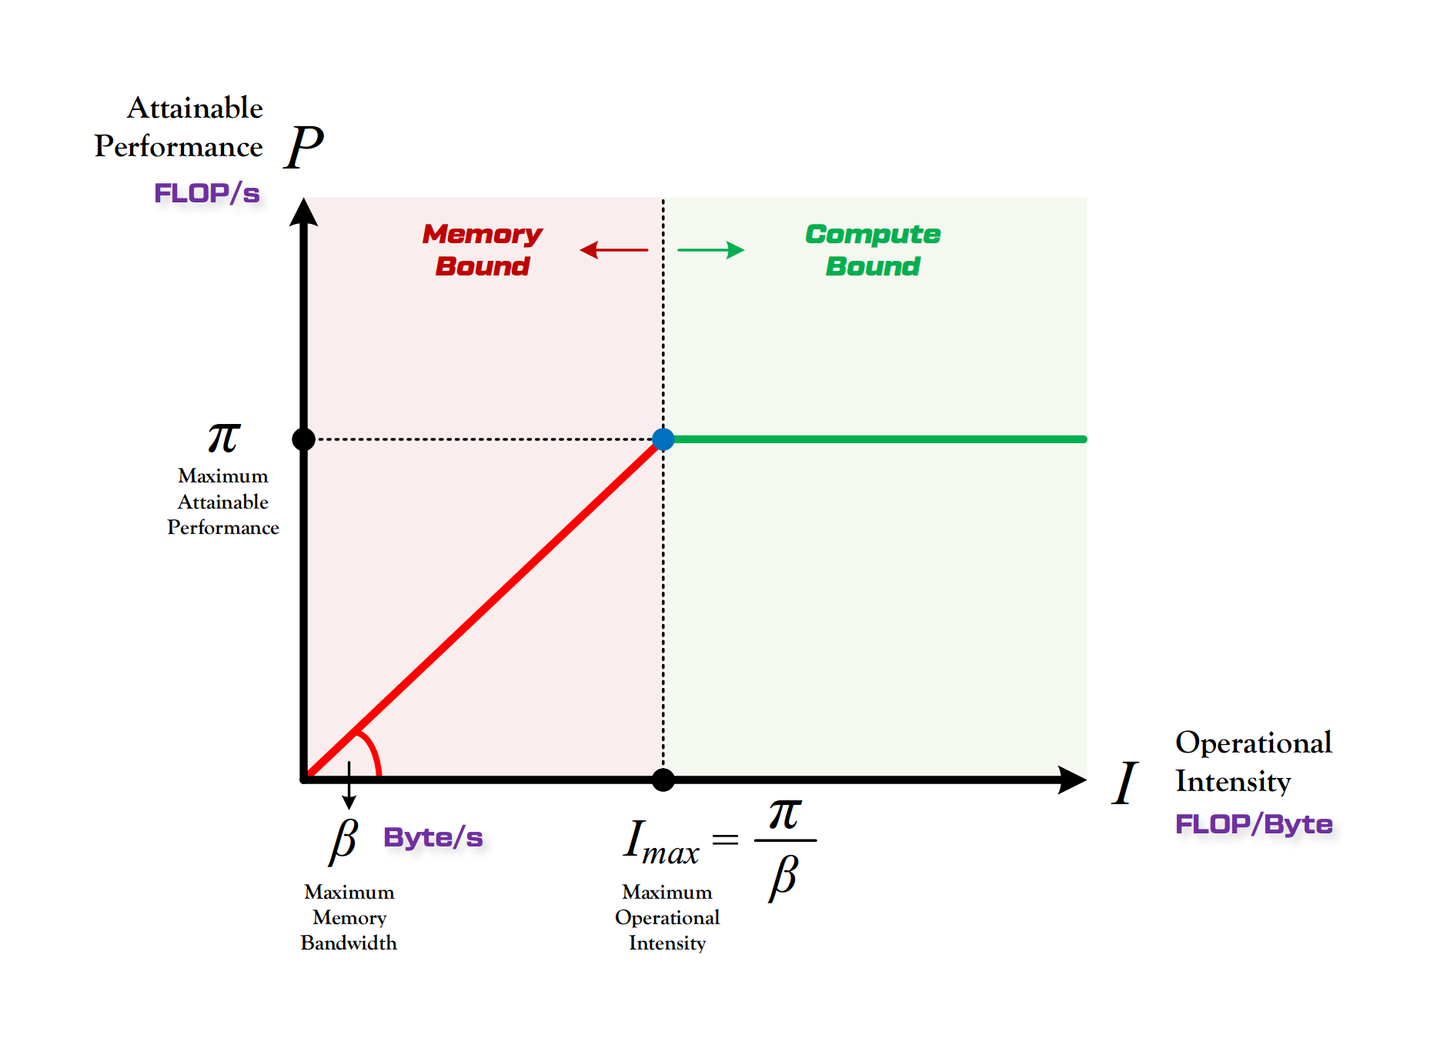
\includegraphics[width=0.7\textwidth]{img/roofline.jpg}
    \end{center}
\end{frame}